\section{What an Object is Made of}
\label{chapter-scenario-template}

\textbf{Created by:} Perawit Charoenwut \\
\textbf{Modified by:}

\subsection*{Scenario Objective}
This scenario illustrates how to represent what materials an object is made of and what its components are using the IOF/BFO ontology framework.

\subsection*{General Pattern Description}
An object may have as parts multiple components or be composed of various materials. Components themselves may also be composed of different materials. In this pattern, an object is related to each of its components via the core:hasComponentPart object property. Both the object and its components are related to the materials from which they are composed via the core:isMadeOf object property. Figure X illustrates this pattern.

For example, an object such as core:Assembly may be composed of multiple components, each made from different materials. In the general case, the parts of an object can be represented using bfo:hasContinuantPart or bfo:hasProperContinuantPart. Both of these relations include a temporal aspect, indicating whether the part–whole relationship holds at all times during the object’s existence or only during a particular period.

When more precise semantics are required to distinguish between a component (a discrete part) and the material from which something is made (a continuous relation), the ontology provides two specialized relations: core:hasComponentPart and core:isMadeOf.

The following two cases demonstrate:

The use of core:isMadeOf alone.

The combined use of core:isMadeOf and core:hasComponentPart.

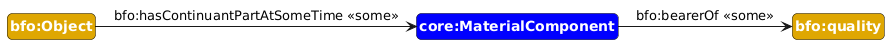
\includegraphics[scale=0.5]{scenarios/object-artifact-material/image/what-is-made-of-schema.png}



\subsection*{Use Case: Buffer}
A buffer is a solution that resists changes in pH by containing a mixture of a weak acid (or weak base) and its corresponding salt, typically dissolved in water.

An acetate buffer is composed of acetic acid (a weak acid) and sodium acetate (its conjugate base), typically in an aqueous solution, and is used to maintain a stable pH in the acidic range, often around pH 4–6. In other words, an acetate buffer is made of three material constituents: water, sodium acetate, and acetic acid.

Because these constituents are dispersed throughout the solution rather than existing as discrete structural parts, the appropriate relation for modeling their composition is core:isMadeOf. Figure X illustrates this pattern along with the following text for the pattern .


\subsection*{Use Case: Buffer Pattern Description}
An acetate buffer can be used in various laboratory procedures to maintain a stable pH in the acidic range. In this scenario, a specific buffer portion (ex:PortionOfAcetateBufferSolution1, a bfo:MaterialEntity) is core:isMadeOf a portion of acetic acid (ex:PortionOfAceticAcid), a portion of sodium acetate (ex:PortionOfSodiumAcetate), and a portion of water (ex:PortionOfWater). The constituent portions instantiate material kinds (ex:AceticAcid, ex:SodiumAcetate, ex:Water), each modeled as a subclass of bfo:MaterialEntity.
This example is chosen to highlight the use of core:isMadeOf for representing a mixture in which constituents are dispersed throughout the whole, as opposed to discrete structural parts modeled with core:hasComponentPart.


\subsection*{Use Case: Packed Chromatography column}
A packed chromatography column consists of a glass chromatography column filled with DEAE–Sepharose resin. The resin comprises a sepharose matrix to which diethylaminoethyl (DEAE) functional groups are covalently attached, enabling anion-exchange separation of biomolecules based on charge.

In ontology terms, the packed chromatography column has as component parts:

A chromatography column that is core:isMadeOf glass.

A DEAE–Sepharose resin that is core:isMadeOf sepharose and core:isMadeOf DEAE.

This pattern illustrates the combined use of core:hasComponentPart to represent discrete structural parts (the column and the resin) and core:isMadeOf to represent the materials from which those parts are composed.

\subsection*{Use Case: Packed Chromatography Column Pattern Description}

A packed chromatography column can be used in biomolecule purification processes to separate components based on charge. In this scenario, the packed chromatography column (ex:PackedChromatographyColumn, a core:MaterialArtifact) core:hasComponentPart a chromatography column (ex:ChromatographyColumn) and a DEAE–Sepharose resin (ex:DEAE-SepharoseResin).

The chromatography column is core:isMadeOf a portion of glass (ex:PortionOfGlass), while the DEAE–Sepharose resin is core:isMadeOf a portion of sepharose (ex:PortionOfSepharose) and core:isMadeOf a portion of diethylaminoethyl molecules (ex:PortionOfDEAEMolecules). The DEAE functional groups are covalently attached to the sepharose matrix, giving the resin its anion-exchange capability.

This example is chosen to illustrate the combined use of core:hasComponentPart for discrete, structural parts (the column and the resin) and core:isMadeOf for the materials from which those parts are composed. In other words, the packed chromatography column core:hasComponentPart its glass column and its resin, while each of these parts is linked to the materials it is composed of via core:isMadeOf.

\subsection*{Use Case Pattern Description}

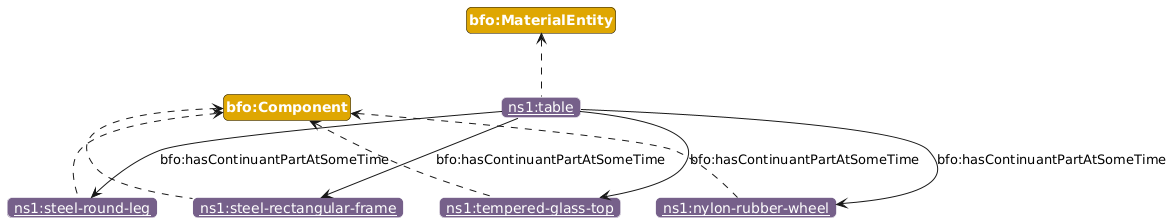
\includegraphics[scale=0.5]{scenarios/object-artifact-material/image/what-is-made-of.png}

The table (ns1:table) is represented as a bfo:MaterialEntity that has four main components:

\begin{itemize}
    \item A tempered glass top (ns1:glass-top)
    \item A stainless steel frame (ns1:steel-frame)component for the frame
    \item Steel legs (ns1:steel-leg)
    \item Nylon wheels (ns1:nylon-wheel)
\end{itemize}

\subsubsection*{Use-Case Example Data}
\begin{table}[h]
% \caption{}
\label{tab:material-components}
\resizebox{\columnwidth}{!}{%
\begin{tabular}{|l|l|l|l|l|l|l|}
\hline
Component ID & Product ID & Component Type & Material & Quality Type & Quality Value & Unit \\ \hline
TOP001 & TABLE001 & Table Top & Tempered Glass & Thickness & 10 & mm \\
TOP001 & TABLE001 & Table Top & Tempered Glass & Area & 0.8 & m² \\
FRAME001 & TABLE001 & Table Frame & Steel & Length & 100 & cm \\
FRAME002 & TABLE001 & Table Frame & Steel & Length & 80 & cm \\
LEG001 & TABLE001 & Table Leg & Steel & Height & 75 & cm \\
LEG001 & TABLE001 & Table Leg & Steel & diameter & 5 & cm \\
WHEEL001 & TABLE001 & Wheel & Nylon & Diameter & 50 & mm \\ \hline
\end{tabular}%
}
\end{table}

\subsubsection*{Data Mapping}


\subsubsection*{Data Validation}
